\documentclass[Orbiter User Manual.tex]{subfiles}
\begin{document}

\section{Basic flight manoeuvres}
\label{sec:basic_flight}
This chapter discusses a few general approaches for manoeuvres during different phases of a flight. Some of the details may differ depending on the spacecraft used, most significantly during launch and landing.


\subsection{Surface flight}
Surface flight paths, as opposed to orbits, include continuously powered trajectories that counter gravitational forces with thrust or aerodynamic lift, as well as suborbital ballistic trajectories with a short initial powered acceleration phase and an unpowered ballistic phase that ends on the surface of the same body. Surface-to-surface transfers (from one surface base to another) typically involve surface flight.\\
Depending on the celestial body, surface flight may take place within an atmosphere. In that case, atmospheric friction will have an influence on the flight parameters, causing atmospheric drag, possibly supersonic effects, surface heating, etc. Some of the vessels in Orbiter are particularly adapted for atmospheric flight, such as the Delta-glider, which has an aerodynamic body and surfaces which generate lift when moving through a planetary surface. The Space Shuttle orbiter makes use of the atmosphere during its reentry and unpowered landing approach to extend its range compared to a capsule, and allow it to land on a runway.\\
In the absence of an atmospheric layer, engine thrust must be substituted for lift to counter gravitational forces. This can be done with dedicated hover thrusters (Delta-glider, Shuttle-A), or with main thrusters, by adjusting the vessel's attitude to provide appropriate horizontal and vertical thrust components. Without an atmosphere to slow the vessel down, orbits can be realised at arbitrarily low altitudes, as long as surface obstacles are cleared. When the horizontal velocity component approaches orbital speed, less vertical thrust is required to maintain altitude.\\
The most useful MFD modes for surface flight are

\begin{itemize}
\item Surface (altitude, speed, acceleration, attitude, atmospheric parameters)
\item HSI (navigation in the presence of VOR beacons, instrument landing)
\item Map (navigation, ground track prediction)
\item VTOL (vertical take-off and landing support)
\end{itemize}


\subsection{Launching into orbit}
\label{ssec:basic_launch}
Launching from a planetary surface into a low orbit is one of the most basic problems in spaceflight. A suitable launch profile minimises fuel consumption, while keeping relevant parameters (acceleration, aerodynamic loads, heat generation, etc.) within predefined limits. The chosen profile will depend on the type of launch vehicle - the Space Shuttle has to follow a precisely defined launch trajectory with little deviation to reach orbit with limited propellant resources and without subjecting its crew to excessive forces at any phase of the ascent, while the futuristic Delta-glider can achieve orbit effortlessly and nearly hands-off. Some general rules can however be formulated:

\begin{itemize}
\item The initial part of the ascent is vertical to leave the denser part of the atmosphere before the increasing airspeed leads to excessive drag and heating.
\item Later the vessel pitches over to start building up the horizontal velocity component required for attaining orbit.
\item The engines may be cut once the highest point of the projected trajectory (\textit{apoapsis}) coincides with the target orbit altitude.
\item Once that point is reached, the engines are engaged again in a \textit{prograde} vessel orientation (aligned with the trajectory direction) for orbital insertion (lifting the lowest part of the orbit above the planet surface and sufficiently high above the atmosphere layer to enter a stable orbit).
\item For efficiency reasons, launch direction should be prograde (in the direction of the planetary rotation, i.e. eastward on Earth) to get the surface velocity component for free. For the same reason, a launch site closer to the equator will be more efficient. (On Earth, a prograde equatorial launch saves $\Delta$v = 930 m/s compared to a retrograde launch).
\item If a specific target orbit must be achieved (e.g. for rendezvous with an orbital station), this will determine a \textit{launch window} (time) and \textit{launch azimuth} (heading). The launch should take place when the launch site passes through the target orbital plane, and the azimuth is given by the inclination of the target plane at the launch latitude. This will minimise the requirement for later expensive orbital pane changes. The \textit{Map} and \textit{Align orbital plane} MFD modes (see sections \ref{ssec:mfd_orbit} and \ref{ssec:mfd_align} respectively) help with picking launch window and azimuth.
\end{itemize}

\noindent
\textbf{Background: Launch azimuth calculation}\\
Given latitude $\phi$ of the launch site and target inclination \textit{i}, the launch azimuth $\beta$ can be calculated with

\[ \beta = \sin^{-1} \frac{\cos i}{\cos \phi} \]

\noindent
This is a simplified formula doesn't take into account the effect of planet rotation. For a discussion of the required correction, see for example the OrbiterWiki (\url{https://www.orbiterwiki.org/wiki/Launch_Azimuth}).


\subsection{Changing the orbit}
\label{ssec:basic_changeorbit}
To change the shape of the orbit without changing the orbital plane, any thrust must be applied in the orbital plane (\textit{in-plane} manoeuvres). An important consideration in orbit changes is the fact that the point in the orbit at which the engines are fired for the orbit change manoeuvre is also part of the new orbit (assuming a short, impulse-like burn). In other words, to modify a particular section of the orbit, the corresponding engine burn should occur on the opposite side of the orbit.\\
\\
\textbf{Task: modifying apoapsis/periapsis distances}\\
A common task is the raising or lowering of apoapsis (highest point of the orbit) or periapsis (lowest point of the orbit), for example for circularising an orbit after initial orbit insertion, or to initialise a change in orbital radius. In keeping with the above principle, the apoapsis distance is modified by an engine burn at periapsis, and vice versa:

\begin{itemize}
\item Increase apoapsis distance: Wait until the ship reaches periapsis. Apply thrust prograde (in the direction of the orbital velocity vector)
\item Decrease apoapsis distance: Wait until the ship reaches periapsis. Apply thrust retrograde (opposite the direction of the orbital velocity vector)
\item Increase periapsis distance: Wait until the ship reaches apoapsis. Apply thrust prograde.
\item Decrease periapsis distance: Wait until the ship reaches apoapsis. Apply thrust retrograde.
\end{itemize}

\noindent
The \textit{Orbit} MFD mode (see section \ref{ssec:mfd_orbit}) can be used to monitor the time to apoapsis and periapsis.  Prograde and retrograde orbit directions can be visualised on the HUD in Orbit mode (see section \ref{ssec:hud_modes}). The vessel can be automatically oriented in prograde or retrograde attitude in preparation for the orbit change burn by using the corresponding RCS attitude modes (see section \ref{ssec:glass_cockpit}).\\
\\
\textbf{Task: Increasing/decreasing the radius of a circular orbit}\\
The manoeuvres in the previous task can be combined to change the radius of a circular orbit. This is achieved by two separate engine burns: the first enters an intermediate elliptic orbit whose apoapsis (or periapsis) distance coincides with the desired orbit radius. The second burn re-circularises the orbit.\\
To raise the radius of the orbit:

\begin{itemize}
\item Turn the ship prograde.
\item Fire main thrusters until apoapsis (at the opposite side of the orbit) reaches the desired orbit radius. Kill thrusters.
\item Wait for half an orbit, until the new apoapsis is reached.
\item Turn prograde again, fire main thrusters until periapsis distance also reaches the desired orbit radius and orbit eccentricity is back to 0.
\end{itemize}

\noindent
To lower the radius of the orbit:

\begin{itemize}
\item As above, but perform both engine burns retrograde instead of prograde.
\end{itemize}

\begin{figure}[H]
	\centering
	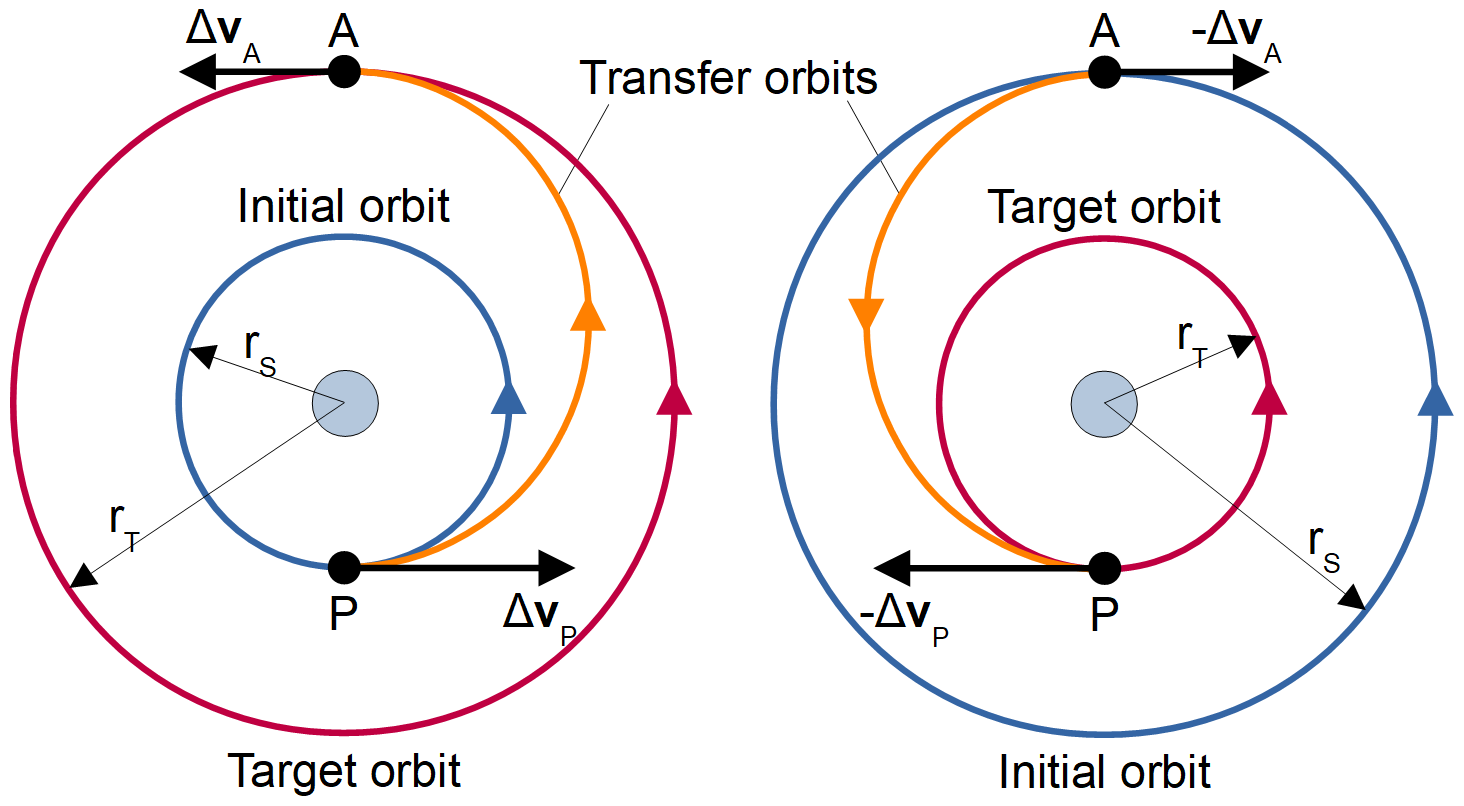
\includegraphics[width=0.75\hsize]{transfer_orbit.png}
	\caption{Moving into a higher orbit involves prograde acceleration at P and A (periapsis and apoapsis of the transfer orbit). Conversely, moving from a higher to a lower orbit requires retrograde acceleration at A and P.}
\end{figure}

\noindent
\textbf{Task: Rotate the argument of periapsis of an elliptic orbit}\\
The task here is to rotate an elliptic orbit in-plane, by moving the apoapsis and periapsis locations without changing the shape of the orbit. One way to accomplish this is by first performing a prograde burn at apoapsis to enter an intermediate circular orbit, then performing a retrograde burn at the desired new apoapsis position to restore the initial elliptic orbit shape. (Alternatively, a retrograde burn at periapsis could be performed, but the required $\Delta v$ budget for these two approaches could be different. Which is cheaper?)\\
Note that the described approach is simple to perform, but may neither be fastest nor cheapest (in terms of fuel consumption). A more direct approach would be to perform the burn at one of the intersections of the old and new orbit, but the computation of burn time and direction is less trivial then.

\begin{figure}[H]
	\centering
	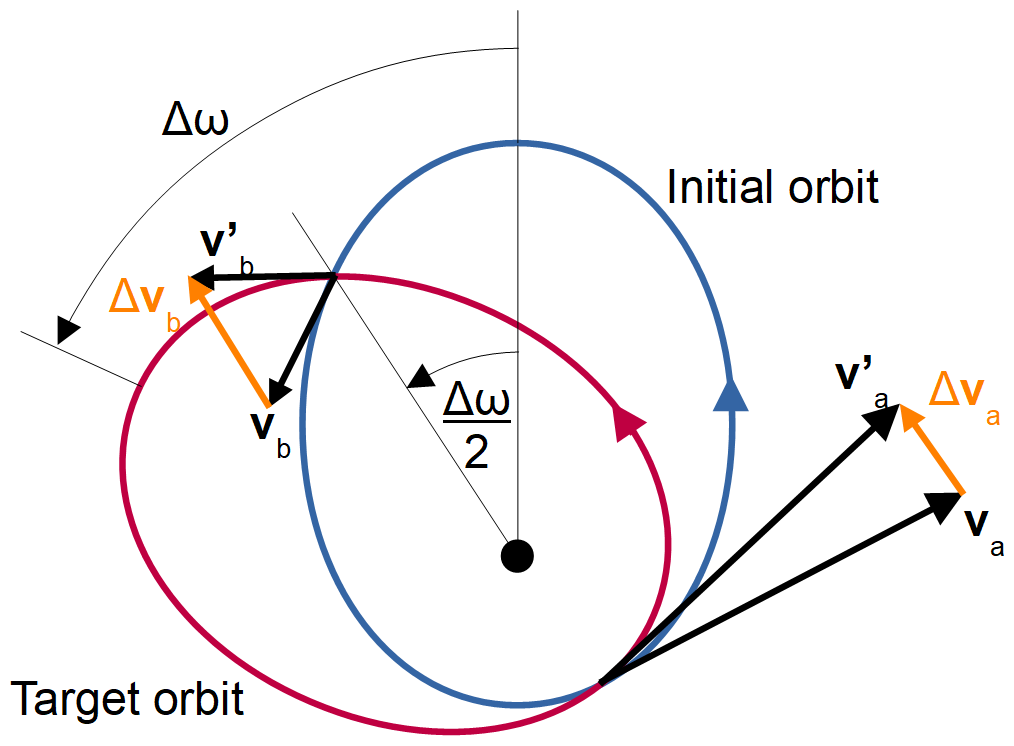
\includegraphics[width=0.5\hsize]{rot_pe.png}
	\caption{Rotation of argument of periapsis by $\Delta\omega$ using a direct burn $\Delta v_{a}$ or $\Delta v_{b}$ at one of the intersection points of initial and target orbits. The burn takes place at true anomaly $v = \Delta\omega / 2$ or $\Delta\omega / 2 + \pi$ in a radial direction.}
\end{figure}


\subsection{Rotating the orbital plane}
\label{ssec:basic_plane}
When trying to rendezvous with another object in orbit, the required orbit changes can be split into two separate phases: a plane change that rotates the plane of the current orbit into that of the target, and further in-plane operations that only require the application of thrust in the plane of the orbit (see previous chapter). Once the orbit planes have been aligned, the remaining operations become essentially two-dimensional, which makes them significantly easier to plan and execute (but possibly less efficient in time and fuel requirements).\\
In terms of the orbital elements, aligning the plane of the orbit with the target plane means to match the two elements which define the orientation of the orbit in space (see section \ref{sec:orb_mech}): inclination (\textit{i}) and longitude of the ascending node ($\Omega$).\\
It should be noted that substantial plane changes can require large $\Delta v$ budgets. It is therefore important to minimise the need for plane changes where possible, for example by carefully planning launch and ascent (launch window and azimuth, see section \ref{ssec:basic_launch}).\\
The rotation of the orbital plane requires the application of out-of-plane thrust, in a direction normal to the current plane. The engine burn takes place in one of the nodes (the points where the orbit crosses the intersection of the current and target planes). This rotates the orbital plane around an axis defined by the current radius vector (which at this point coincides with the line of nodes).

\begin{figure}[H]
	\centering
	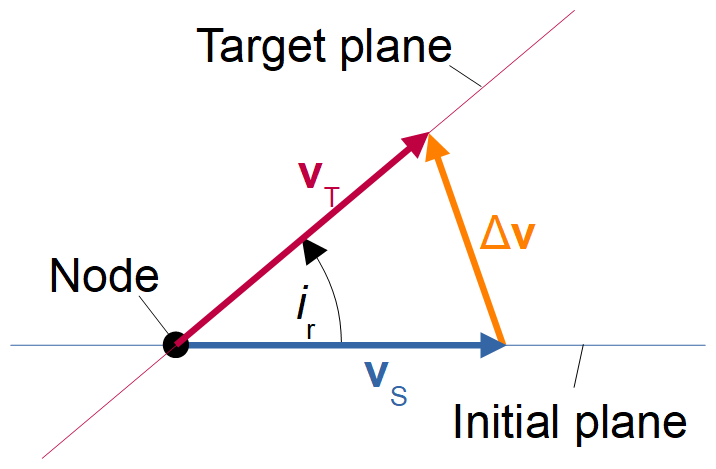
\includegraphics[width=0.5\hsize]{plane_change_dv.png}
\end{figure}

\noindent
The amount of normal $\Delta v$ required to rotate by a given angle $i_{r}$ is proportional to the orbital velocity \textit{v}. It is therefore more fuel-efficient to perform the plane change where \textit{v} is small, i.e. at the node closest to apoapsis. You may be able to save even more fuel (at the cost of additional time requirements) by first raising apoapsis with a separate in-plane manoeuvre, because the fuel saved from the more efficient plane change more than makes up for the additional in-plane burns.\\
\\
\textbf{Notes:}

\begin{itemize}
\item If the angle between the initial and target plane is large it may be necessary to adjust the orientation of the spacecraft during the burn to keep it normal to the plane. Alternatively (and slightly more efficient), the spacecraft may be kept at a constant orientation given by the mean of the normals of the initial and target planes.
\item Substantial plane changes require long burns. It may not be possible to align the plane in a single node crossing. If the inclination difference does not decrease further during the burn, cut the engines and wait for the next node crossing.
\item Since the manoeuvre will take a finite amount of time $\Delta T$, thrusters should be engaged approximately $\Delta T$/2 before the node encounter.
\end{itemize}

\noindent
The direction of the burn depends on the node at which it takes place. If we define the normal vector \textbf{n}$_{s}$ as

\[ \textbf{n}_{s} = \textbf{r}_{s} \times \textbf{v}_{s} \]

\noindent
for radius vector $\textbf{r}_{s}$ and velocity vector $\textbf{v}_{s}$, then the thrust should be applied in direction +$\textbf{n}_{s}$ ("normal") at the descending node (DN) and in direction -$\textbf{n}_{s}$ ("anti-normal") at the ascending node (AN).

\begin{figure}[H]
	\centering
	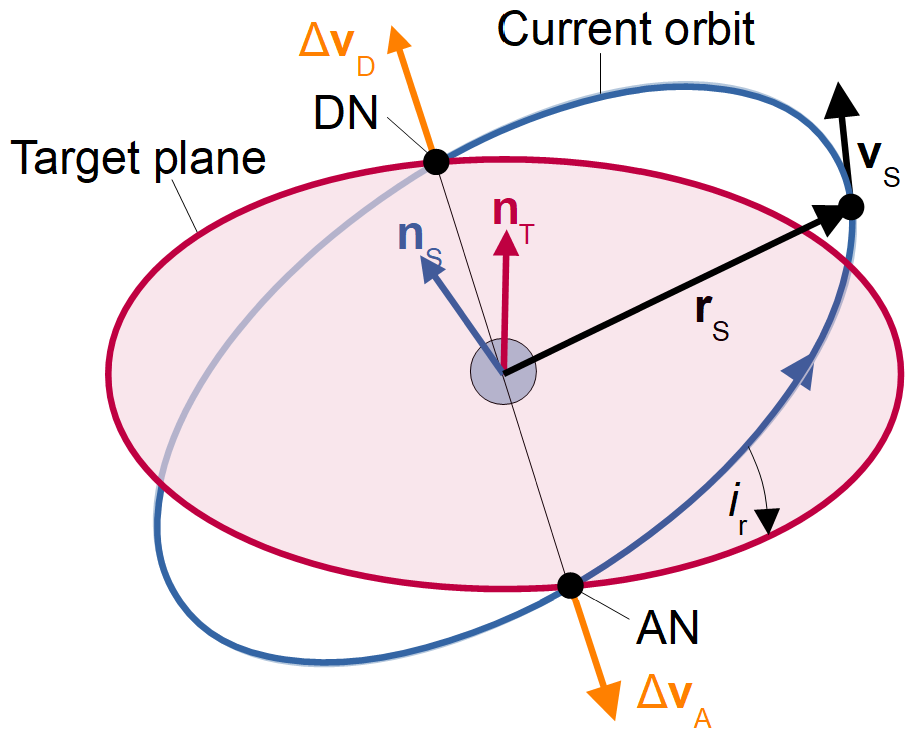
\includegraphics[width=0.5\hsize]{plane_change.png}
	\caption{Alignment of the orbital plane requires an out-of-plane burn at one of the nodes. $\textbf{r}_{S}$: radius vector, $\textbf{v}_{S}$: orbital velocity vector, AN: ascending node, DN: descending node, $\textbf{n}_{S}$: normal of the current plane, $\textbf{n}_{T}$: normal of the target plane.}
\end{figure}

\noindent
\textbf{In practice:}

\begin{itemize}
\item The \textit{Align orbital plane} MFD mode (see section \ref{ssec:mfd_align}) is designed to aid in plane alignment. Make sure the display is in Orbit mode (\Shift\keystroke{M}) and select the target object (\Shift\keystroke{T}).
\item The HUD should be in \textit{Orbit} mode. As the ship approaches a node (intersection with the target plane), use the appropriate RCS attitude mode to rotate to a normal (\keystroke{;}) at DN or anti-normal (\keystroke{'}) orientation to the orbital plane at AN. Use the HUD Orbit inclination ladder to monitor progress.
\item As soon as the time-to-burn (TtB) counter reaches 0 for the targeted node and the burn indicator ([BURN]) is shown, engage full main engines. This will happen when the time to node (TtN) counter reaches half the estimated burn time (BT).
\item Make sure that the relative inclination (RInc) decreases, i.e. that the rate (R) is negative, otherwise you may be pointing in the wrong direction.
\item Adjust the ship's orientation as required to keep normal to the orbital plane (the automated RCS mode will do this for you).
\item Cut engines when:

\begin{itemize}
\item relative inclination (RInc) reaches 0, or
\item rate (R) turns positive, or
\item burn time (BT) counts down to 0, or
\item burn indicator ([BURN]) disappears.
\end{itemize}

\item If the relative inclination was not sufficiently reduced, repeat the procedure at the next node passage.
\item During the manoeuvre make sure that your orbit does not become unstable. Watch in particular for the eccentricity and periapsis altitude (use the Orbit MFD mode to monitor this).
\end{itemize}


\subsection{Synchronising orbits}
\label{ssec:basic_sync}
The next step in a rendezvous manoeuvre after aligning the orbital planes (see previous chapter) is to modify the orbit in-plane such that it intercepts the target's orbit and both ship and target arrive simultaneously at the interception point. Use the \textit{Synchronise Orbit} MFD mode to calculate the appropriate orbit changes.\\
For simplicity we first assume that the ship and target are in a circular orbit with the same orbital radius (for modifying orbital radii see section \ref{ssec:basic_changeorbit}), i.e. both objects have the same orbital elements except for the mean anomaly. The method for intercepting the target is then as follows:

\begin{itemize}
\item Switch the reference mode of the Synchronise Orbit MFD to \textit{Manual} and rotate the axis to your current position.
\item Turn your ship \textit{prograde} (using Orbit HUD mode and RCS attitude functions) and fire main thrusters.
\item The orbit will become elliptic, with an increasing apoapsis distance. Your current position becomes periapsis of the new orbit. Simultaneously the orbit period and the times to reference axis are increasing.
\item Kill engines as soon as one of the ship-time-to-reference (Sh-ToR) times coincides with one of the target-time-to-reference (Tg-ToR) times.
\item Wait until the target is intercepted (the corresponding Sh-ToR and Tg-ToR times have counted down).
\item Fire thrusters retrograde to get back to the circular orbit and match velocity with the target.
\end{itemize}

\begin{figure}[H]
	\centering
	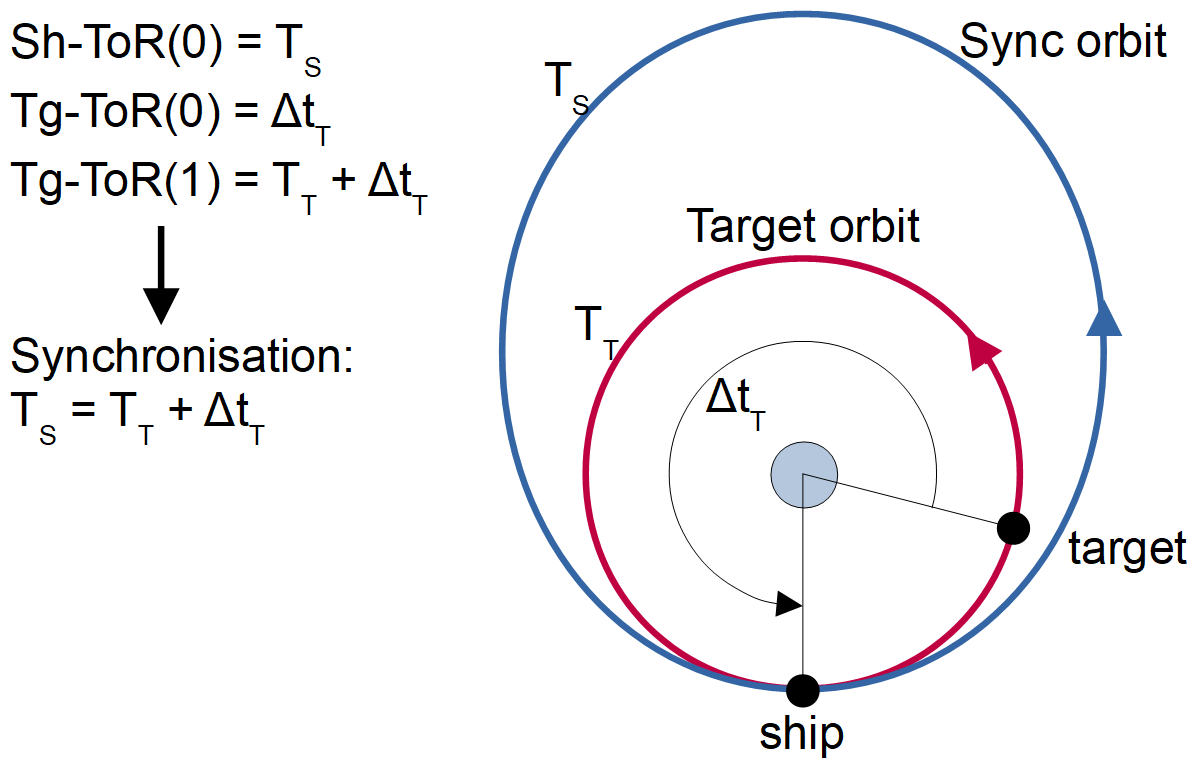
\includegraphics[width=0.5\hsize]{transition_orbit.png}
	\caption{A transition orbit to intercept the target at the next periapsis passage. T$_{T}$: target orbit period, T$_{S}$: transition orbit period, $\Delta$t$_{T}$: remaining time for target to reach periapsis from its current position.}
\end{figure}

\noindent
\textbf{Notes:}

\begin{itemize}
\item Instead of increasing the apoapsis distance one could fire retrograde and reduce the periapsis distance in this manoeuvre. This may be more efficient if the target is ahead of the ship. However the maximum orbit change in this case is limited by keeping periapsis at a safe altitude.
\item There is usually a trade-off between the time to encounter and the required orbit change ($\Delta v$ budget). An encounter in an earlier orbit may require longer engine burns to enter and exit the transition orbit. Matching the intercept times in a later orbit requires shorter burns.
\item It is not essential that the orbits are identical or circular at the start of the manoeuvre. It is sufficient for them to intersect. In that case it is best to use \textit{Intersection 1} or \textit{2} reference mode in Synchronise MFD mode.
\item You don't necessarily need to wait until you reach the reference point before firing thrusters, but it simplifies matters because otherwise the intersection point itself will move, making the alignment of orbit timings more difficult.
\end{itemize}


\subsection{Docking}
\label{ssec:basic_docking}
Docking to an orbital station is the final step in a rendezvous manoeuvre. Assuming that the target station has been intercepted following the operations discussed in the preceding chapters (i.e. ship and target are in close proximity in similar orbits), the last task is to actually dock at one of the station's available docking ports. This requires

\begin{itemize}
\item positioning the ship on the approach path to the selected port
\item orienting the ship so that its docking port is aligned with the target
\item approaching the docking port along the approach path with suitable relative velocity, correcting for lateral and rotational drift along the way
\end{itemize}

\noindent
Here is a checklist of the steps involved in the docking operation:

\begin{itemize}
\item Select \textit{Docking} mode for one of the MFD instruments (\Shift\keystroke{F1}, \Shift\keystroke{D}).
\item Tune one of your NAV receivers to the station's long-range transponder (XPDR) frequency, using the COM/NAV MFD mode (\Shift\keystroke{F1}, \Shift\keystroke{C}). Tune a second receiver to the IDS (instrument docking system) frequency of the intended docking port. The transponder and IDS frequencies for all vessels are listed in the object info dialog (\Ctrl\keystroke{I}).
\item Link the Docking MFD display to the XPDR signal by selecting the corresponding NAV receiver (\Shift\keystroke{N}).
\item Copy the docking parameters to the HUD by pressing the HUD button of the Docking MFD (\Shift\keystroke{H}).
\item If not done already, null out relative velocity with the target by rotating the ship to align it with the negative relative velocity marker ($\odot$) and fire main thrusters until the indicated velocity value (V) approaches zero.
\item Rotate the ship to face the station (D[ISS]$\vartriangleright$ marker).
\item Approach the station to about 10 km and hold at that relative position. Switch the Docking MFD display over to the IDS receiver (\Shift\keystroke{N}) and copy to the HUD (\Shift\keystroke{H}). This will activate alignment indicators in the MFD display, and a visual representation of the approach path (rectangles) in the HUD.
\item Move towards the approach path rectangle furthest from the station, and hold.
\item Align the ship's orientation with the flight path direction using the '$\times$' indicator in the MFD. Use RCS thrusters in \textit{rotational} (ROT) mode for this.
\item Align the ship's rotation along its longitudinal axis (bank angle) using the arrow indicator in the MFD display.
\item Align the ship's position on the approach path using the '+' indicator in the MFD. Switch RCS to \textit{linear} (LIN) mode for this.
\item Approach the station by using the longitudinal RCS thrusters in linear mode (\keystroke{6}/\keystroke{9}$_{Num}$). During approach correct your lateral deviation from approach path continuously with linear RCS. Correct rotational drift with rotational RCS.
\item Slow down approach speed to less than 0.1 m/s before contact with the station's docking port.
\item Wait until positive docking confirmation is reported.
\item To disengage from the docking port, press \Ctrl\keystroke{D}.
\end{itemize}

\begin{figure}[H]
	\centering
	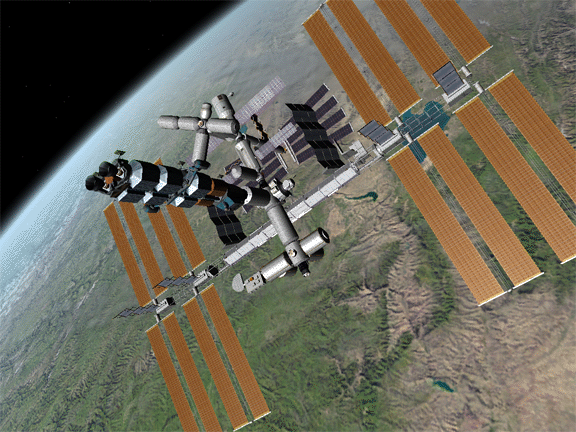
\includegraphics[width=0.75\hsize]{shuttlea_iss.png}
	\caption{A Shuttle-A class cargo ship after successfully completed docking approach to the ISS.}
\end{figure}

\noindent
\textbf{Notes:}

\begin{itemize}
\item For precise attitude control with the keyboard, use the RCS thrusters in low power mode (\Ctrl + Numpad key).
\item Rotational alignment is not currently enforced, but may be in future versions.
\item Currently no collision tests are performed, so you might fly straight through the station if you miss the docking approach.
\end{itemize}

\noindent
\textbf{Docking adapter location:}\\
If the ship's docking adapter is not mounted along its longitudinal axis, you will need to approach the station with your ship rotated accordingly. An example is the Space Shuttle, which had its docking adapter (if present) installed in the payload bay. In this case, the pilot may not have a direct view of the station, but the Docking MFD alignment cues will still work correctly. Care must be taken to use the correct RCS thrusters for alignment corrections.\\
\\
\textbf{Docking at rotating stations:}\\
Stations like Orbiter's fictional Luna-OB1 rotate to use centrifugal forces for emulating gravity - which is nice for its inhabitants but makes docking a lot more complicated. Docking is only possible along the rotation axis, so at most 2 docking ports can be provided. The docking procedure is similar to the standard one, but once aligned with the approach path, the rotation around the ship's longitudinal axis must be synced with that of the station. Some points to note:

\begin{itemize}
\item Initiate your ship's longitudinal rotation only immediately before docking (when past the last approach rectangle). Once you are rotating, linear adjustments become very difficult.
\item Once the rotation is matched with the station, don't hit \textit{Kill Rot} (\keystroke{5}$_{Num}$) by accident, or you will have to start the rotation alignment again.
\end{itemize}


\subsection{Lunar and interplanetary transfers}
A spaceflight from Earth to the Moon or a planet is generally performed in several phases:

\begin{itemize}
\item Launch from Earth's surface into a low Earth orbit
\item Ejection burn from orbit into a cis-lunar or interplanetary transfer orbit
\item If required, one or several mid-course correction burns
\item Orbit injection burn from transfer orbit into an orbit around the target object
\item If part of the mission, a de-orbit burn and descent to the surface by a landing module
\end{itemize}

\noindent
The Moon and the planets orbit in planes close to the ecliptic (the plane of Earth's orbit). It therefore simplifies mission planning if the spacecraft's initial Earth orbit is also aligned with the plane of the ecliptic. This avoids the need for out-of-plane manoeuvres.\\
\\
\textbf{Hohmann transfer}\\
A common type of interplanetary transfer is the Hohmann orbit, an elliptic orbit with periapsis at the initial (circular) Earth orbit, and apoapsis at the target planet's distance from Earth. This requires a prograde orbit ejection burn at the appropriate time, similar to the orbit change manoeuvre described in section \ref{ssec:basic_changeorbit}. The launch window is restricted by the requirement that the spacecraft and target body arrive at the transfer orbit's apoapsis location at the same time. Within that window, the transfer orbit ejection burn takes place at the spacecraft's appropriate position in its Earth orbit, to make use of its orbital velocity. In Orbiter, the Transfer MFD mode (see section \ref{ssec:mfd_transfer}) assists with simple transfer planning. For more complex missions, the TransX MFD (see section \ref{ssec:mfd_transx}) is also included in Orbiter.


\begin{figure}[H]
	\centering
	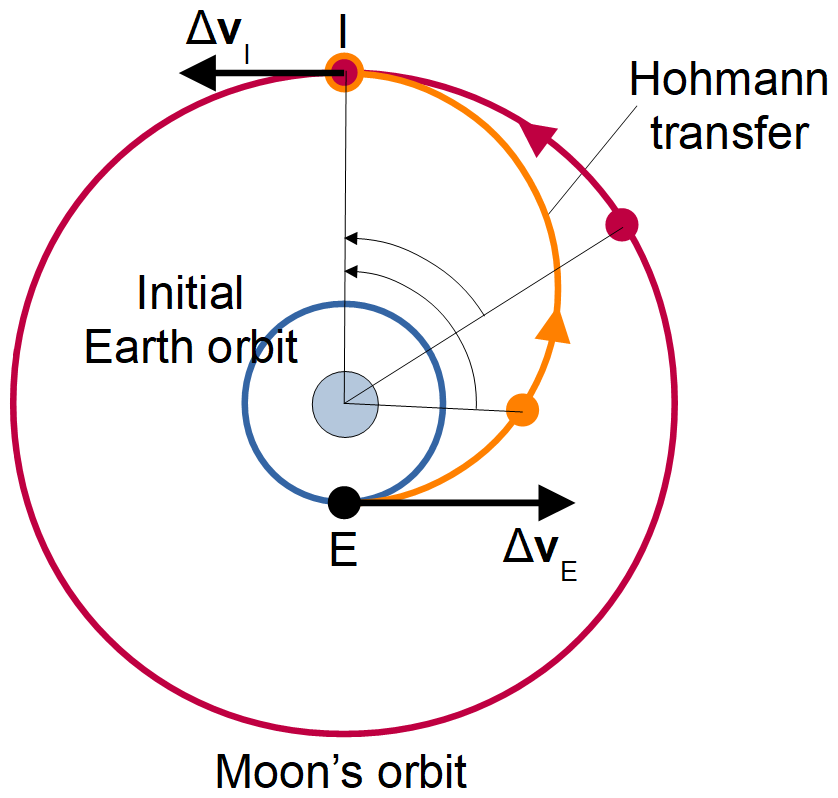
\includegraphics[width=0.5\hsize]{hohmann.png}
	\caption{A Hohmann transfer from Earth orbit to a Moon encounter. E: ejection burn for transition to transfer orbit. I: Lunar encounter, orbit injection burn.}
\end{figure}

\noindent
\textbf{Gravity assist}\\
Interplanetary transfers often make use of gravity-assist manoeuvres ("slingshots") around other planets to increase velocity and shorten flight times. Slingshots, in particular if they involve multiple planetary encounters, require careful planning.\\
\\
\textbf{Free return trajectories}\\
On arriving at the target body, an orbit injection burn is required to enter an orbit around the body from the transfer orbit. It is however sometimes possible to design the transfer orbit such that the spacecraft returns to Earth after swinging around the target body if the injection burn is not executed. This approach was used by the early Apollo lunar missions in case the lunar orbit injection burn failed. Free return trajectories are also possible for Mars missions.


\subsection{Landing (runway approach)}
\label{ssec:basic_landing}
Some of Orbiter's spacecraft support powered or unpowered runway approaches, similar to normal aircraft. Examples are the Delta-glider and the Space Shuttle. The Shuttle Landing Facility (SLF) at Kennedy Space Center provides a good opportunity for exercising landing approaches.\\
\\
\textbf{Visual approach indicators}\\
The visual approach aids at SLF are designed for Shuttle landings. They include a Precision Approach Path Indicator (PAPI) for long-range glide slope alignment, and a Visual Approach Slope Indicator (VASI) for short-range alignment. The PAPI is set up for a glide slope of 20° (about 6 times as steep as standard aircraft approach slopes!). The VASI is set up for a 1.5° slope during the final flare up prior to touchdown.\\
\\
\textbf{Precision Approach Path Indicator:} The PAPI consists of an array of 4 lights, which appear white or red to the pilot depending on the approaching vessel's position above or below the glide slope. At the correct slope there will be 2 white and 2 red lights (see figure below). In Orbiter there are 2 PAPI units per approach direction at the SLF, located about 2000 m in front of the runway threshold.

%\begin{table}[H]
	%\centering
	\begin{longtable}{ |p{0.12\textwidth} p{0.25\textwidth}| }
	\hline\rule{0pt}{2ex}
	
\includegraphics[width=0.1\textwidth, margin=0pt 1ex 0pt 1ex, valign=m]{papi_1.png} & Above glide slope\\
	\hline\rule{0pt}{2ex}
	
\includegraphics[width=0.1\textwidth, margin=0pt 1ex 0pt 1ex, valign=m]{papi_2.png} & Slightly above glide slope\\
	\hline\rule{0pt}{2ex}
	
\includegraphics[width=0.1\textwidth, margin=0pt 1ex 0pt 1ex, valign=m]{papi_3.png} & On glide slope\\
	\hline\rule{0pt}{2ex}
	
\includegraphics[width=0.1\textwidth, margin=0pt 1ex 0pt 1ex, valign=m]{papi_4.png} & Slightly below glide slope\\
	\hline\rule{0pt}{2ex}
	
\includegraphics[width=0.1\textwidth, margin=0pt 1ex 0pt 1ex, valign=m]{papi_5.png} & Below glide slope\\
	\hline
	\end{longtable}
%\end{table}

\noindent
\textbf{Visual Approach Slope Indicator:} The VASI consists of a red bar of lights and a set of white lights in front of it. At the correct slope, the white lights are aligned with the red bar (see figure below). At the SLF, the VASI is located 670 m behind the runway threshold.

%\begin{table}[H]
	%\centering
	\begin{longtable}{ |p{0.12\textwidth} p{0.25\textwidth}| }
	\hline\rule{0pt}{2ex}
	
\includegraphics[width=0.1\textwidth, margin=0pt 1ex 0pt 1ex, valign=m]{vasi_1.png} & Above glide slope\\
	\hline\rule{0pt}{2ex}
	
\includegraphics[width=0.1\textwidth, margin=0pt 1ex 0pt 1ex, valign=m]{vasi_2.png} & On glide slope\\
	\hline\rule{0pt}{2ex}
	
\includegraphics[width=0.1\textwidth, margin=0pt 1ex 0pt 1ex, valign=m]{vasi_3.png} & Below glide slope\\
	\hline
	\end{longtable}
%\end{table}

\begin{figure}[H]
	\centering
	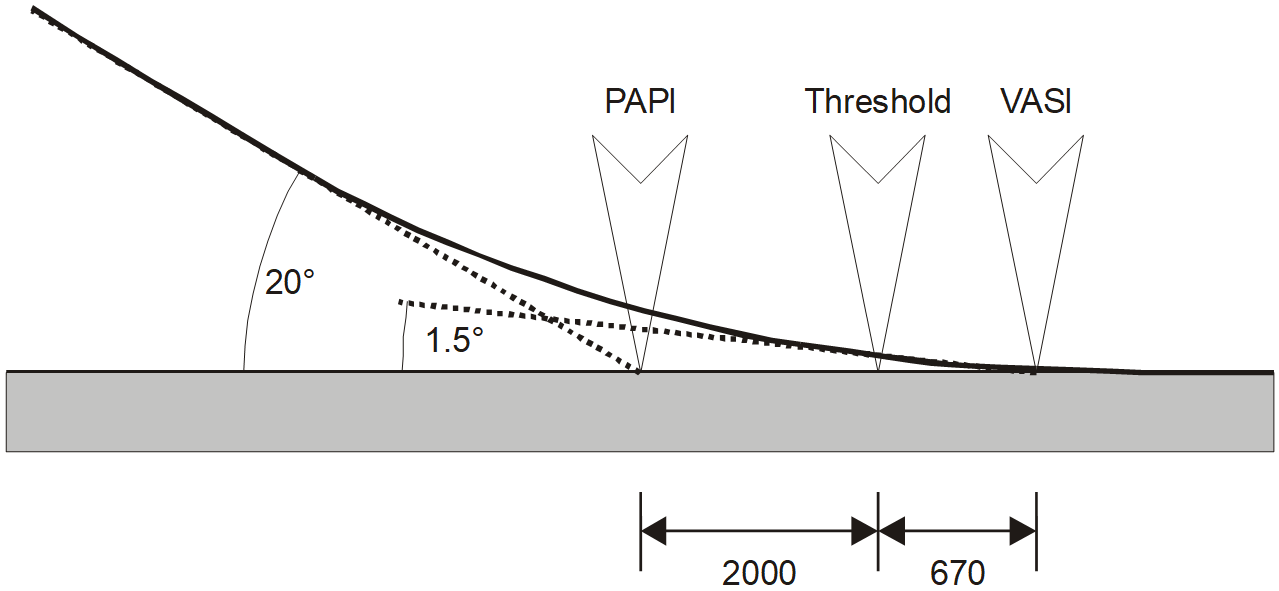
\includegraphics[width=0.75\hsize]{shuttle_approach.png}
	\caption{SLF Shuttle approach path}
\end{figure}

\noindent
\textbf{Instrument landing system (ILS)}\\
Runways equipped with ILS transmit a radio signal that provides alignment data to an approaching spacecraft. This information can be presented to the pilot in the HSI MFD mode (see section \ref{ssec:mfd_hsi}) or in dedicated instruments such as the Delta-glider's VOR indicator instrument. To get ILS data, tune one of the NAV receivers to the desired ILS frequency and switch the HSI feed to that receiver. ILS frequencies can be found in the surface base info pages (\Ctrl\keystroke{I}).

\begin{figure}[H]
	\centering
	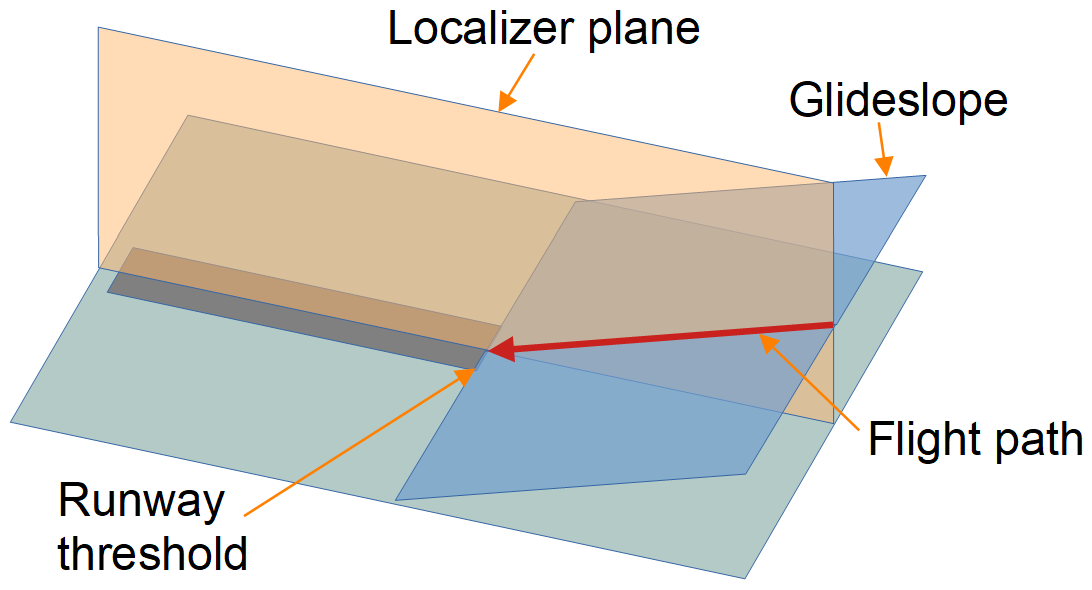
\includegraphics[width=0.5\hsize]{ils_planes.png}
\end{figure}

\noindent
In ILS mode, the course select needle is fixed to the runway approach direction. The central section of the needle acts as a course deviation bar (CDI). Horizontal alignment is achieved when the course needle points to the 12 o'clock direction and the CDI is centred.\\
Vertical alignment is indicated with the glideslope needle. This horizontal bar symbolises the position of the target approach plane relative to the spacecraft at the current distance to the runway threshold. The spacecraft is on glideslope when the needle is centred in the instrument display. A low approach is represented with the needle above the centre line, a high approach with the needle below centre.

\begin{figure}[H]
	\centering
	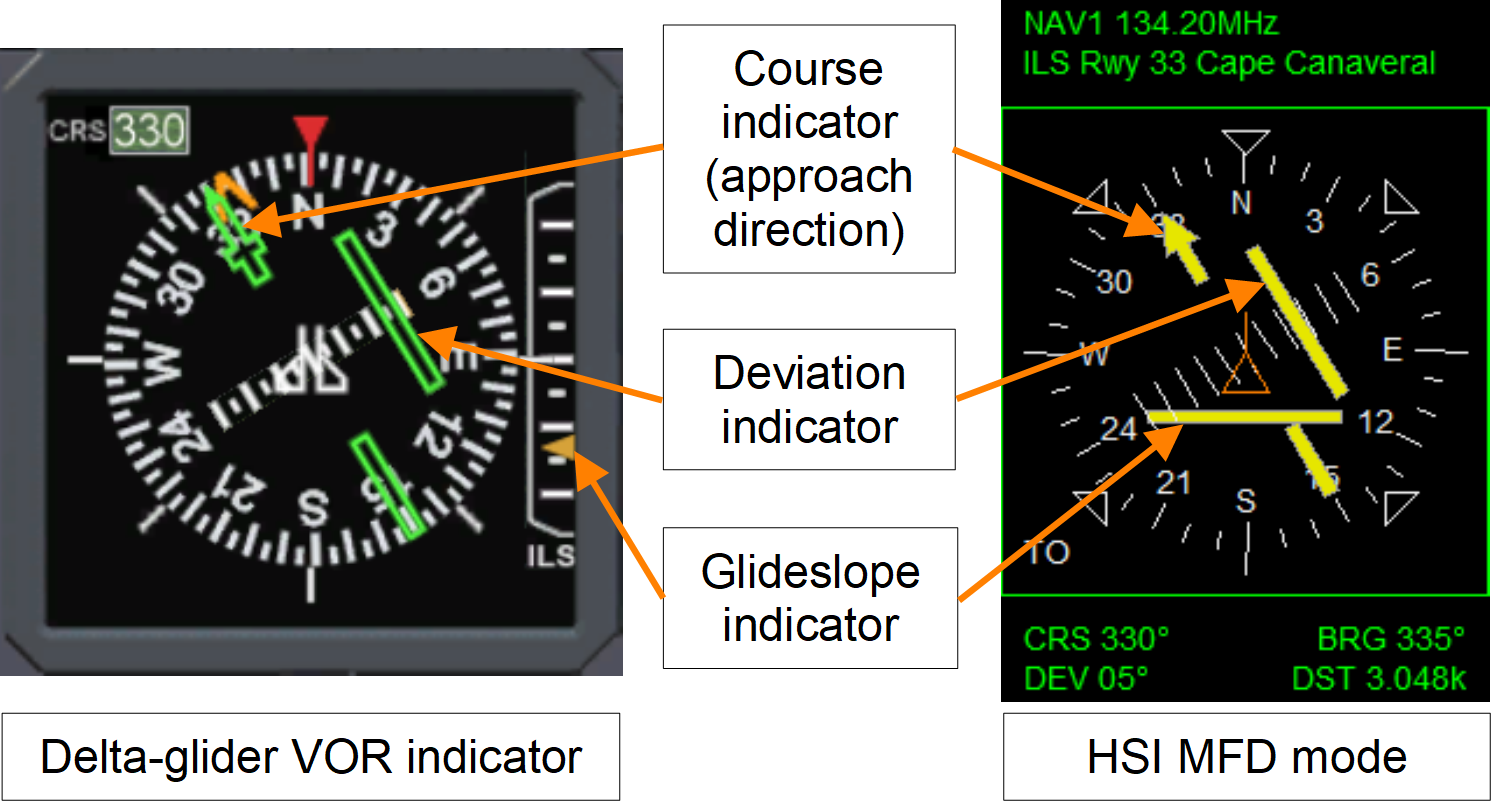
\includegraphics[width=0.75\hsize]{ils_instruments.png}
	\caption{HSI instruments in ILS mode. Left: DG VOR indicator, right: HSI MFD mode.}
\end{figure}

\end{document}
